\section{Data Fusion and Preprocessing}\label{section:fusion}

This section introduces the process of processing the raw data received from the sensors and creating a final representation of the environment that is further used as an input for the other stages of the process.\par
In this thesis, we receive colored 2-dimensional images from an HD camera and a raw 3D point cloud from a 3D LiDAR sensor. The goal is to use these two inputs and generate a colored point cloud for a more accurate environment representation.\par
In this work, we assume that both sensors are calibrated and that the excentric parameters, namely field of view and transformation matrix between sensor's frames, are already known. If this is not the case, some of the following well-known techniques \cite{Calibration1} \cite{Calibration2} can be used for their determination.\par
The whole process can be divided into three major parts. In the beginning, the frequencies of the sensors must be synchronized. Then, after the input data are synchronized, the data fusion is performed, and the individual scene representations are merged into one mutual model, containing information from all individual sensors. Finally, the built representation is preprocessed and simplified by removing the unnecessary data, especially the information about the ground. The whole process is visualized in Figure \ref{fig:dataFusionWorkflow} and each step is described in the following subsections.

\begin{figure}[htpb]
    \centering
    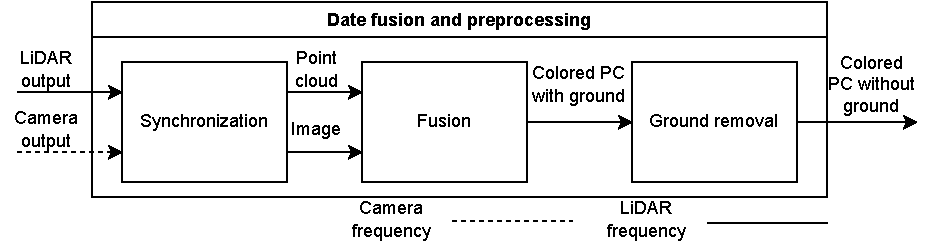
\includegraphics[width=0.8\textwidth]{dataFusionWorkflow.pdf}
    \caption{Data fusion workflow} \label{fig:dataFusionWorkflow}
\end{figure}

Figure \ref{fig:dataFusionExample} illustrates example inputs received from the sensors, generated output after the data fusion, and final generated output after the ground removal.

\begin{figure}[!tbp]
    \centering
    \subfloat[Input received from the camera.]{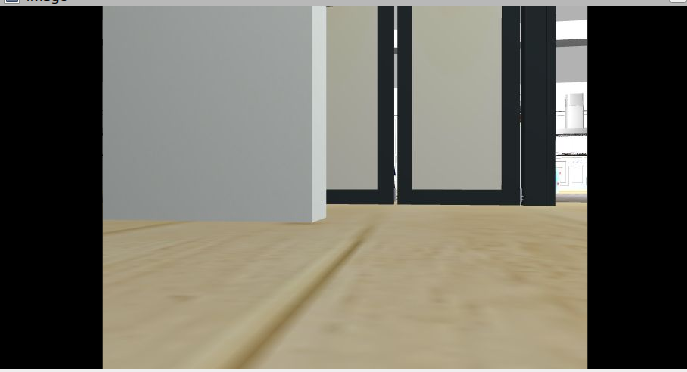
\includegraphics[height=0.2\textheight]{dataFusionExampleImage.png}\label{fig:dataFusionExample1}}
    \hfill
    \subfloat[Input received from the LiDAR.]{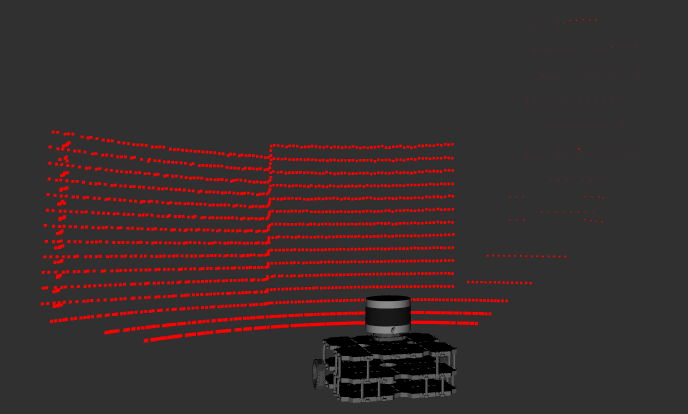
\includegraphics[height=0.2\textheight]{dataFusionExampleRawCloud.png}\label{fig:dataFusionExample2}}
    \\
    \subfloat[Colored point cloud after data fusion]{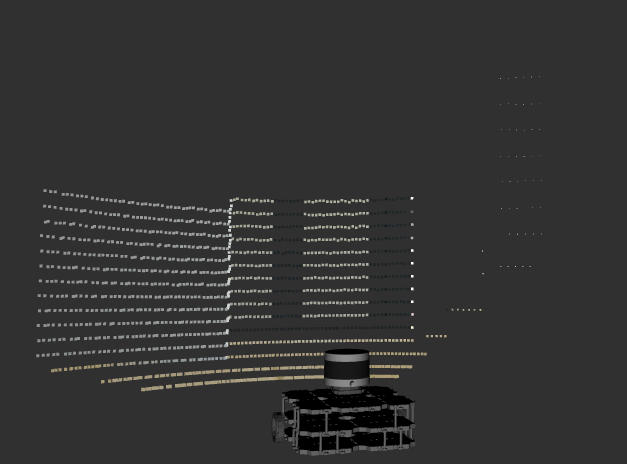
\includegraphics[height=0.2\textheight]{dataFusionExampleColoredCloud.png}\label{fig:dataFusionExample3}}
    \hfill
    \subfloat[Final result after the ground removal]{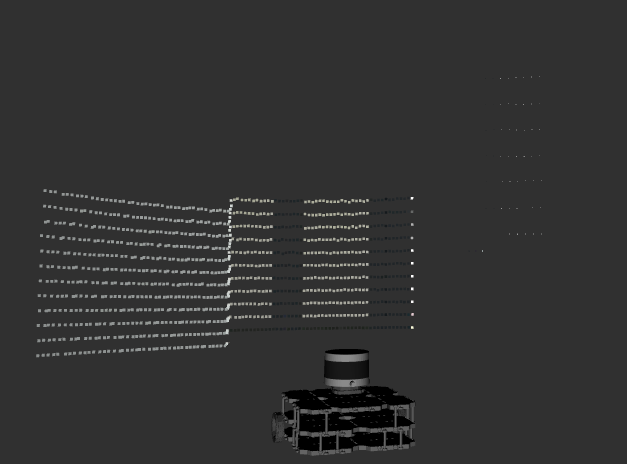
\includegraphics[height=0.2\textheight]{dataFusionExampleFinal.png}\label{fig:dataFusionExample4}}
    \caption{Data fusion sensors inputs and generated outputs after each stage}
    \label{fig:dataFusionExample}
\end{figure}

\subsection{Sensors Synchronization}

This section solves the problem that the sensors deliver data at different times with different frequencies. The goal of the synchronization is to receive unsynchronized data from both sensors and return synchronized pairs of images and point clouds that will be used for further fusion.\par
The technique used in this thesis is based on the assumption that the camera frequency is significantly larger than the frequency of the 3D-LiDAR\footnote{In the experiments, we used a camera that has 15 times higher frequency than the 3D-LiDAR.}. Based on this fact, the system can just record all the images received from the camera. All point clouds received from the 3D-LiDAR are afterward paired with the last received image.\par
The time difference between the image and point cloud is so low, compared to the frequency of the LiDAR, that it can be neglected, and we can assume that the image and the point cloud were taken simultaneously.

\subsection{Data Fusion}

At this point, we assume that all the data are synchronized and working with a pair of images and raw point clouds representing the same scene at the same time. The goal is to build a colored 3D point cloud.\par
The point cloud $PC$ is represented as an unordered set of triples, describing a single point's $x, y, z$ coordinates:
$$
    PC \subseteq \left\{ (x,y,z) | (x,y,z) \in \mathbb{R}^3\right\}.
$$
The image can be represented as a function $img: \mathbb{R}^2 \rightarrow \mathbb{N}_0^3 \cup \{0\}$ taking $x,y$ pixel coordinates as input and returning RGB representation of the pixels color or 0, if the give coordinates are out of range\footnote{If $x$ or $y$ are not the whole numbers, they are rounded to the nearest whole number.}:
$$
    img(x,y) = \begin{cases}
        (r,g,b) & \text{if $(x,y)$ are inside of the cameras field of view} \\
        0       & \text{otherwise,}
    \end{cases}
$$
where $r,g,b$ corresponds to the pixel color's red, green, and blue parts.\par
The result $CPC$ will be represented as an unordered set of sextuplets, describing a single point's $x, y, z$ coordinates together with $r, g, b$ colors:
$$
    CPC \subseteq \left\{ (x,y,z,r,g,b) | (x,y,z,r,g,b) \in \mathbb{R}^3 \times \mathbb{N}_0^3 \right\}.
$$\par
Let $\mathbf{P}$ be the projection matrix that projects 3D world coordinates into the 2D pixel coordinates on the image plane using the following formula:
$$
    \mathbf{x} = \mathbf{P}\mathbf{X},
$$
where $\mathbf{X} = \left[x_\text{world},y_\text{world},z_\text{world}\right]^T$ represents a 3D world coordinates vector and $\mathbf{x} = \left[x_\text{image}, y_\text{image}\right]^T$ represents a 2D image plane coordinates vector. This matrix can be found using the camera's and LiDAR's excentric parameters received from the calibration. \cite{pinholeCitation}\par
If we know the projection matrix $\mathbf{P}$, we can iterate through all the points in the point cloud, project them into the image plane, find the corresponding pixel and bind its color with the examined point. All points outside the camera's field of view shall be ignored and not included in the result.\par
The algorithm for the fusion of the data received from LiDAR and camera is summarized in the Algorithm \ref{alg:fusion}.

\begin{algorithm}
    \caption{LiDAR and camera data fustion}\label{alg:fusion}
    \begin{algorithmic}
        \Require Point cloud $PC$, camera image $img$
        \Ensure Colored point cloud $CPC$
        \State $CPC := \{\}$  \Comment{Initialize result as an empty set}
        \State $\mathbf{P} \leftarrow $ build projection matrix
        \For{$(x,y,z) \in PC$} \Comment{Iterate through all points in $PC$}
        \State $[x_i,y_i]^T \leftarrow  \mathbf{P}\cdot[x,y,z]^T$ \Comment{Project current point to the image plane}
        \If{$img(x_i,y_i) \neq 0$} \Comment{Ignore points out of cameras field of view}
        \State $(r,g,b) \leftarrow  img(x_i,y_i)$  \Comment{Get projected pixel color}
        \State $CPC \leftarrow CPC \cup \{(x,y,z,r,g,b)\}$  \Comment{Add colored point to the result}
        \EndIf
        \EndFor
        \State\Return $CPC$
    \end{algorithmic}
\end{algorithm}

\subsection{Ground Removal}

Ground removal is a widely used technique, applied by many algorithms working with 3D point clouds. Even if the information about the ground, particularly about the ground color, might help distinguish between two different scenes, the points representing the floor are usually in the same position for every scene and therefore carry a relatively small information value. Removing these points can significantly reduce the input size, with minimal loss of the information value, which can positively influence the algorithm's performance. Furthermore, the ground points may connect two completely separate objects and therefore have a negative influence on the scene segmentation or object detection algorithms.\par
Let's assume that all points from the point cloud are represented in the world's frame of reference and that $y$ axis is orthogonal to the ground. Then, it is evident that there exists a threshold $y_{th}$, such that all points representing a ground have $y$ coordinate lower or equal to the $y_{th}$ and all other points will have $y$ coordinate larger than $y_{th}$. So, if the threshold $y_{th}$ is known\footnote{This threshold can be very easily determined experimentally.}, the ground point can be removed simply by filtering the points by their $y$ coordinate. The ground removal process is summarized in the Algorithm \ref{alg:groundRemoval}.

\begin{algorithm}
    \caption{Ground removal}\label{alg:groundRemoval}
    \begin{algorithmic}
        \Require Colored point cloud $CPC$, threshold $y_{th}$
        \Ensure Colored point cloud $CPC_2$ without ground
        \State $CPC_2 := \{\}$  \Comment{Initialize result as an empty set}
        \For{$(x,y,z,r,g,b) \in CPC$} \Comment{Iterate through all points in $CPC$}
        \If{$y > y_{th}$} \Comment{Ignore points under the threshold}
        \State $CPC_2 \leftarrow CPC_2 \cup \{(x,y,z,r,g,b)\}$  \Comment{Add current point to the result}
        \EndIf
        \EndFor
        \State\Return $CPC_2$
    \end{algorithmic}
\end{algorithm}

Besides the ground, this method can remove some other objects' bottom parts, like the feet of pedestrians, wheels of wheelchairs, etc., which can lead to a slightly more significant information loss than pure ground removal. However, there exist other, better ground removal techniques, usually based on machine learning, which do not suffer from this issue \cite{groundRemoval1} \cite{groundRemoval2}. Yet, these techniques typically require more computational resources than the simple filtering approach, and the results are usually not significantly different\footnote{Especially in the indoor environments with static objects like furniture, which are in the main focus of this work}, so we decided to prefer this simple method despite the minor quality drawbacks.